\documentclass[14pt]{extbook}
\usepackage{multicol, enumerate, enumitem, hyperref, color, soul, setspace, parskip, fancyhdr} %General Packages
\usepackage{amssymb, amsthm, amsmath, latexsym, units, mathtools} %Math Packages
\everymath{\displaystyle} %All math in Display Style
% Packages with additional options
\usepackage[headsep=0.5cm,headheight=12pt, left=1 in,right= 1 in,top= 1 in,bottom= 1 in]{geometry}
\usepackage[usenames,dvipsnames]{xcolor}
\usepackage{dashrule}  % Package to use the command below to create lines between items
\newcommand{\litem}[1]{\item#1\hspace*{-1cm}\rule{\textwidth}{0.4pt}}
\pagestyle{fancy}
\lhead{Makeup Progress Quiz 3}
\chead{}
\rhead{Version C}
\lfoot{1648-1753}
\cfoot{}
\rfoot{Summer C 2021}
\begin{document}

\begin{enumerate}
\litem{
Construct the lowest-degree polynomial given the zeros below. Then, choose the intervals that contain the coefficients of the polynomial in the form $x^3+bx^2+cx+d$.\[ 5 + 2 i \text{ and } 1 \]\begin{enumerate}[label=\Alph*.]
\item \( b \in [-18, -7], c \in [35.4, 40.7], \text{ and } d \in [-30.8, -28.8] \)
\item \( b \in [-6, 7], c \in [-10.4, -5.5], \text{ and } d \in [2.6, 6.3] \)
\item \( b \in [-6, 7], c \in [-4.6, -2.6], \text{ and } d \in [-4.2, 2.7] \)
\item \( b \in [10, 12], c \in [35.4, 40.7], \text{ and } d \in [24.9, 29.1] \)
\item \( \text{None of the above.} \)

\end{enumerate} }
\litem{
Describe the end behavior of the polynomial below.\[ f(x) = 7(x - 4)^{3}(x + 4)^{4}(x - 8)^{2}(x + 8)^{2} \]\begin{enumerate}[label=\Alph*.]
\begin{multicols}{2}\item 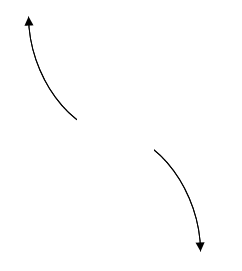
\includegraphics[width = 0.3\textwidth]{../Figures/polyEndBehaviorAC.png}\item 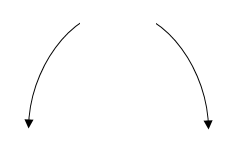
\includegraphics[width = 0.3\textwidth]{../Figures/polyEndBehaviorBC.png}\item 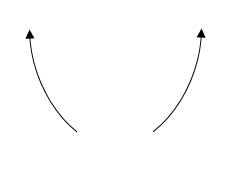
\includegraphics[width = 0.3\textwidth]{../Figures/polyEndBehaviorCC.png}\item 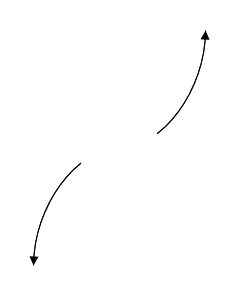
\includegraphics[width = 0.3\textwidth]{../Figures/polyEndBehaviorDC.png}\end{multicols}\item None of the above.
\end{enumerate} }
\litem{
Describe the end behavior of the polynomial below.\[ f(x) = 4(x + 3)^{2}(x - 3)^{7}(x + 8)^{5}(x - 8)^{6} \]\begin{enumerate}[label=\Alph*.]
\begin{multicols}{2}\item 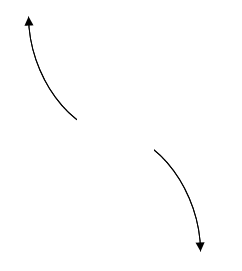
\includegraphics[width = 0.3\textwidth]{../Figures/polyEndBehaviorCopyAC.png}\item 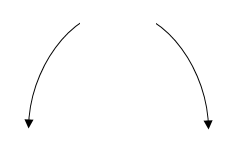
\includegraphics[width = 0.3\textwidth]{../Figures/polyEndBehaviorCopyBC.png}\item 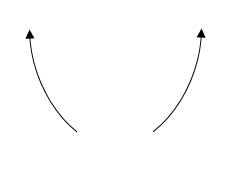
\includegraphics[width = 0.3\textwidth]{../Figures/polyEndBehaviorCopyCC.png}\item 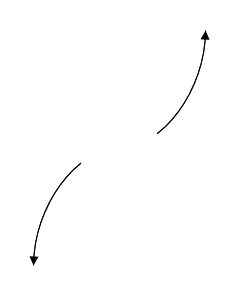
\includegraphics[width = 0.3\textwidth]{../Figures/polyEndBehaviorCopyDC.png}\end{multicols}\item None of the above.
\end{enumerate} }
\litem{
Construct the lowest-degree polynomial given the zeros below. Then, choose the intervals that contain the coefficients of the polynomial in the form $ax^3+bx^2+cx+d$.\[ \frac{-3}{4}, -7, \text{ and } \frac{-1}{3} \]\begin{enumerate}[label=\Alph*.]
\item \( a \in [12, 14], b \in [94, 98], c \in [90, 105], \text{ and } d \in [20, 26] \)
\item \( a \in [12, 14], b \in [-99, -94], c \in [90, 105], \text{ and } d \in [-26, -20] \)
\item \( a \in [12, 14], b \in [-93, -88], c \in [31, 33], \text{ and } d \in [20, 26] \)
\item \( a \in [12, 14], b \in [78, 86], c \in [-43, -37], \text{ and } d \in [-26, -20] \)
\item \( a \in [12, 14], b \in [94, 98], c \in [90, 105], \text{ and } d \in [-26, -20] \)

\end{enumerate} }
\litem{
Describe the zero behavior of the zero $x = -9$ of the polynomial below.\[ f(x) = 2(x - 4)^{10}(x + 4)^{6}(x + 9)^{10}(x - 9)^{7} \]\begin{enumerate}[label=\Alph*.]
\begin{multicols}{2}\item 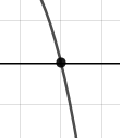
\includegraphics[width = 0.3\textwidth]{../Figures/polyZeroBehaviorAC.png}\item 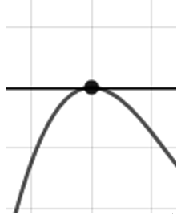
\includegraphics[width = 0.3\textwidth]{../Figures/polyZeroBehaviorBC.png}\item 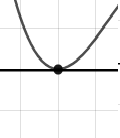
\includegraphics[width = 0.3\textwidth]{../Figures/polyZeroBehaviorCC.png}\item 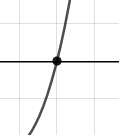
\includegraphics[width = 0.3\textwidth]{../Figures/polyZeroBehaviorDC.png}\end{multicols}\item None of the above.
\end{enumerate} }
\litem{
Which of the following equations \textit{could} be of the graph presented below?
\begin{center}
    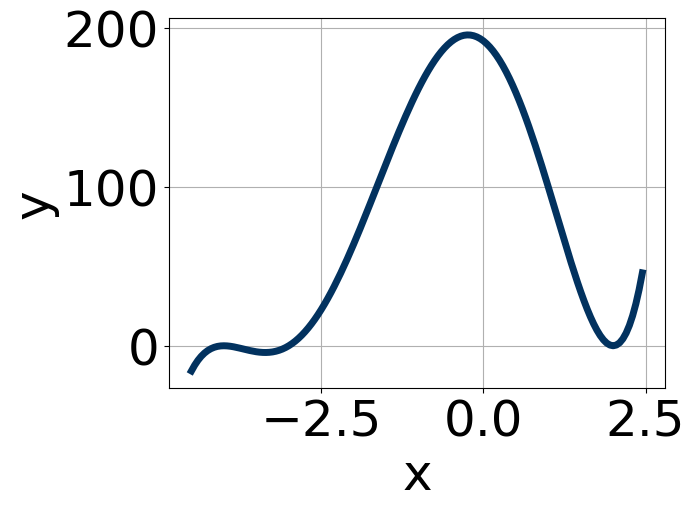
\includegraphics[width=0.5\textwidth]{../Figures/polyGraphToFunctionC.png}
\end{center}
\begin{enumerate}[label=\Alph*.]
\item \( 15(x + 4)^{6} (x - 2)^{7} (x + 3)^{5} \)
\item \( -6(x + 4)^{10} (x - 2)^{6} (x + 3)^{8} \)
\item \( 17(x + 4)^{10} (x - 2)^{7} (x + 3)^{10} \)
\item \( -19(x + 4)^{8} (x - 2)^{8} (x + 3)^{7} \)
\item \( 6(x + 4)^{4} (x - 2)^{8} (x + 3)^{7} \)

\end{enumerate} }
\litem{
Construct the lowest-degree polynomial given the zeros below. Then, choose the intervals that contain the coefficients of the polynomial in the form $x^3+bx^2+cx+d$.\[ 2 + 3 i \text{ and } 1 \]\begin{enumerate}[label=\Alph*.]
\item \( b \in [-1.8, 1.9], c \in [-4.15, -3.21], \text{ and } d \in [2.99, 3.53] \)
\item \( b \in [-9.1, -3.5], c \in [16.78, 18.65], \text{ and } d \in [-14.03, -11.89] \)
\item \( b \in [4.7, 5.3], c \in [16.78, 18.65], \text{ and } d \in [11.64, 13.41] \)
\item \( b \in [-1.8, 1.9], c \in [-3.38, -1.37], \text{ and } d \in [1.75, 2.85] \)
\item \( \text{None of the above.} \)

\end{enumerate} }
\litem{
Describe the zero behavior of the zero $x = -4$ of the polynomial below.\[ f(x) = 6(x - 4)^{7}(x + 4)^{12}(x + 3)^{4}(x - 3)^{6} \]\begin{enumerate}[label=\Alph*.]
\begin{multicols}{2}\item 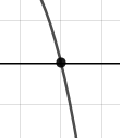
\includegraphics[width = 0.3\textwidth]{../Figures/polyZeroBehaviorCopyAC.png}\item 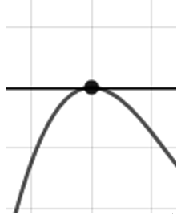
\includegraphics[width = 0.3\textwidth]{../Figures/polyZeroBehaviorCopyBC.png}\item 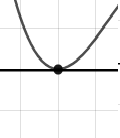
\includegraphics[width = 0.3\textwidth]{../Figures/polyZeroBehaviorCopyCC.png}\item 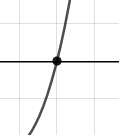
\includegraphics[width = 0.3\textwidth]{../Figures/polyZeroBehaviorCopyDC.png}\end{multicols}\item None of the above.
\end{enumerate} }
\litem{
Construct the lowest-degree polynomial given the zeros below. Then, choose the intervals that contain the coefficients of the polynomial in the form $ax^3+bx^2+cx+d$.\[ \frac{1}{2}, \frac{5}{4}, \text{ and } \frac{-1}{5} \]\begin{enumerate}[label=\Alph*.]
\item \( a \in [37, 43], b \in [-63, -59], c \in [10, 12], \text{ and } d \in [4, 9] \)
\item \( a \in [37, 43], b \in [-24, -15], c \in [-38, -26], \text{ and } d \in [-12, -4] \)
\item \( a \in [37, 43], b \in [-63, -59], c \in [10, 12], \text{ and } d \in [-12, -4] \)
\item \( a \in [37, 43], b \in [74, 85], c \in [38, 41], \text{ and } d \in [4, 9] \)
\item \( a \in [37, 43], b \in [55, 66], c \in [10, 12], \text{ and } d \in [-12, -4] \)

\end{enumerate} }
\litem{
Which of the following equations \textit{could} be of the graph presented below?
\begin{center}
    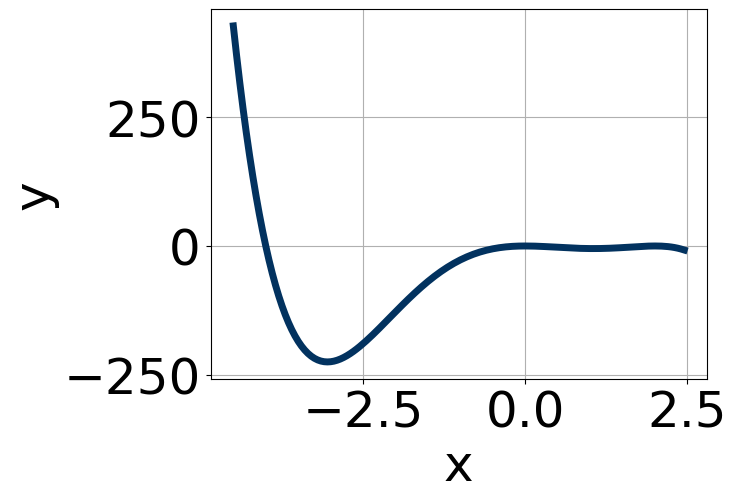
\includegraphics[width=0.5\textwidth]{../Figures/polyGraphToFunctionCopyC.png}
\end{center}
\begin{enumerate}[label=\Alph*.]
\item \( -2x^{8} (x - 1)^{5} (x + 2)^{7} \)
\item \( 13x^{9} (x - 1)^{4} (x + 2)^{9} \)
\item \( -14x^{8} (x - 1)^{7} (x + 2)^{10} \)
\item \( 4x^{4} (x - 1)^{11} (x + 2)^{11} \)
\item \( 7x^{8} (x - 1)^{6} (x + 2)^{7} \)

\end{enumerate} }
\end{enumerate}

\end{document}